\section{Динамика}
%TODO Добавить задачи на системы блоков + задачи Черепанова
 
\begin{ex}
На наклонной поверхности с углом $\alpha$ к горизонту находится брусок. 
Коэффициент трения бруска о поверхность равен $\mu$. С каким ускорением будет двигаться брусок?
\begin{ans}
если $\mu > \tan \alpha$, то $a = 0$; если $\mu < \tan \alpha$, то $a = g(\sin \alpha - \mu \cos \alpha)$.
\end{ans}
\end{ex}

\begin{ex}
\hspace{0pt} \\
\begin{minipage}{.65\textwidth}
(2005) Между двумя неподвижными муфтами может без трения перемещаться вверх и вниз стержень, масса которого $m$. Стержень нижним концом касается гладкой поверхности клина массой $M$. Клин лежит на гладком горизонтальном столе. Определите ускорения стержня и клина.
\end{minipage}
\begin{minipage}{.35\textwidth}
\centering
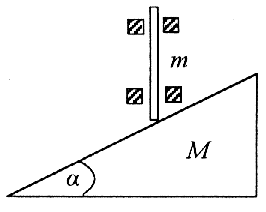
\includegraphics[width = 0.9 \textwidth]{ConnectedInclinedRod.png}
\end{minipage}
\begin{ans}
$a_1 = g \frac{m \sin^2 \alpha}{m \sin^2 \alpha + M \cos^2 \alpha}$, $a_2 = g\frac{m \sin \alpha \cos \alpha}{m \sin^2 \alpha + M \cos^2 \alpha}$
\end{ans}
\end{ex}

\begin{ex}
Клин высотой $h$ с углом наклона $\alpha$ стоит на гладкой горизонтальной поверхности. Масса клина $m_1$. С вершины клина начинает соскальзывать без трения брусок массой $m_2$. Найдите ускорение клина и время соскальзывания бруска.
\begin{ans}
$a_1 = g \frac{m_2 \sin \alpha \cos \alpha}{m_1 + m_2 \sin^2 \alpha}$, $t=\sqrt{\frac{2h(m_1+m_2\sin^2\alpha)}{(m_1+m_2)g \sin^2 \alpha}}$
\end{ans}
\end{ex}

\begin{ex}
(2015) Брусок скользит по длинной наклонной плоскости с углом наклона $\alpha = 30^{\circ}$, движущейся равномерно относительно земли по горизонтальной поверхности со скоростью $u = 10$ м/с в направлении противоположном вершине с углом $\alpha$. Начальная скорость бруска относительно плоскости равна нулю, коэффициент трения бруска о плоскость $\mu = 0,4$. 1) Определите минимальную скорость бруска относительно земли. 2) Через какое время скорость бруска относительно земли будет равна 10 м/с? 3) По какой траектории будет двигаться брусок относительно земли?
\begin{ans}
$v_{min} = u \sin \alpha = 5$ м/c, $t = v_2/g(\sin \alpha - \mu \cos \alpha) = 11,3$ с, парабола.
\end{ans}
\end{ex}

\begin{ex}
\hspace{0pt} \\
\begin{minipage}{.65\textwidth}
Брусок массы $m$ тянут за нить так, что он движется с постоянной скоростью по
горизонтальной плоскости с коэффициентом трения $\mu$. Найти угол $\alpha$, при котором натяжение нити минимально. Чему оно равно?
\end{minipage}
\begin{minipage}{.35\textwidth}
\centering
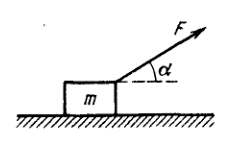
\includegraphics[width = 0.9 \textwidth]{MinForceAngle.png}
\end{minipage}
\begin{ans}
$\tan \alpha = \mu$, $F = \mu mg / \sqrt{\mu^2 + 1}$
\end{ans}
\end{ex}

\begin{ex}
По наклонной плоскости, образующей угол $\alpha$ с горизонтом, за веревку вытягивают ящик массы $m$. 
Коэффициент трения ящика о плоскость равен $\mu$. Под каким углом $\beta$ к горизонту следует тянуть веревку, 
чтобы равномерно двигать ящик с наименьшим усилием? Каково это усилие?
\begin{ans}
$\tan \beta = \mu$, $F = mg \sin (\alpha + \beta)$ при $\alpha + \ beta < \pi/2$, иначе $F = mg$.
\end{ans}
\end{ex}

\begin{ex}
(2016) Брусок массой 10 кг положили на наклонную плоскость с углом наклона к горизонту $\alpha = 30^{\circ}$. Коэффициент трения между бруском и плоскостью равен $\mu = 0,8$. 1) Докажите, что брусок будет покоиться относительно плоскости. 2) Определите минимальную горизонтальную силу, направленную вдоль наклонной плоскости и перпендикулярно плоскости рисунка, которую нужно приложить к бруску, чтобы его сдвинуть. 3) Определите минимальную силу‚ которую нужно приложить к бруску для того, чтобы перемещать его вверх по наклонной плоскости.
\begin{center}
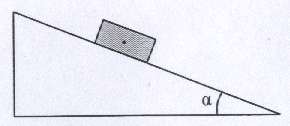
\includegraphics[width = 0.4\textwidth]{InclinedSurfaceFriction.png}
\end{center}
\begin{ans}
$F_2 = mg \sqrt{(\mu \cos \alpha)^2 - (\sin \alpha)^2} = 48$ Н, $F_3 = mg(\mu \cos \alpha + \sin \alpha)/\sqrt{\mu^2 + 1} = 93,1$ Н. 
\end{ans}
\end{ex}

\begin{ex}
\hspace{0pt} \\
\begin{minipage}{.65\textwidth}
При какой максимальной силе $F$ верхний брусок еще не будет скользить по нижнему? Массы брусков $m_1$ и $m_2$, коэффициент трения между ними $\mu$, поверхность стола гладкая.
\end{minipage}
\begin{minipage}{.35\textwidth}
\centering
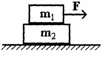
\includegraphics{0403DynamicsBlocks.jpg}
\end{minipage}
\begin{ans}
$F = \mu m_1 g \left(m_1/m_2 + 1 \right)$
\end{ans}
\end{ex}

\begin{ex}
\hspace{0pt} \\
\begin{minipage}{.65\textwidth}
Листы бумаги, сложенные, как показано на рисунке, склеивают свободными концами через лист таким образом, что получаются две самостоятельные кипы $A$ и $B$. Вес каждого листа 0.06 Н, число всех листов 200, коэффициент трения бумаги о бумагу, а также о стол, на котором бумага лежит, равен 0.2. Предполагая, что одна из кип удерживается неподвижно, определить наименьшее горизонтальное усилие $F$, необходимое для того, чтобы вытащить вторую кипу.
\end{minipage}
\begin{minipage}{.35\textwidth}
\centering
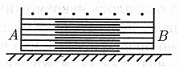
\includegraphics[width = 0.9 \textwidth]{0402DynamicsPaper.jpg}
\end{minipage}
\begin{ans}
$F = $
\end{ans}
\end{ex}

\begin{ex}
\hspace{0pt} \\
\begin{minipage}{.65\textwidth}
По вертикально подвешенному в поле тяжести Земли кольцу радиуса $R$ может скользить без трения шарик массы $m$. 
В начальный момент времени кольцо неподвижно, и шарик находится в нижней точке кольца. 
Как будет двигаться шарик, если кольцо начнет вращаться вокруг вертикальной оси с угловой скоростью $\omega$?
\end{minipage}
\begin{minipage}{.35\textwidth}
\centering
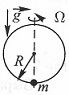
\includegraphics{0405DynamicsRing.jpg}
\end{minipage}
\begin{ans}
$\cos \alpha = g/\omega^2 R$, при $g < \omega^2 R$, иначе $\alpha = 0$.
\end{ans}
\end{ex}

\begin{ex}
\hspace{0pt} \\
\begin{minipage}{.65\textwidth}
К вершине прямого кругового конуса с помощью нити длиной $L$ прикреплена небольшая шайба. Вся система вращается вокруг оси конуса, расположенной вертикально. При каком числе оборотов в единицу времени шайба не будет отрываться от поверхности конуса? Угол при вершине конуса $2\alpha$.
\end{minipage}
\begin{minipage}{.35\textwidth}
\centering
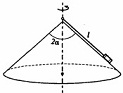
\includegraphics{0406DynamicsCone.jpg}
\end{minipage}
\begin{ans}
$\nu = \frac{1}{2\pi}\sqrt{\frac{g}{L \cos \alpha}}$
\end{ans}
\end{ex}

\begin{ex}
У края диска радиусом $R$ лежит монета. Диск раскручивается так, что его угловая скорость линейно растет со временем по закону $\omega = \varepsilon t$.  В какой момент времени монета слетит с диска, если коэффициент трения между диском и монетой равен $\mu$? Какой угол с направлением к центру диска образует сила трения в этот момент?
\begin{ans}
При $\varepsilon < \mu g /R$ $t=\frac{1}{\sqrt{\varepsilon}}\left( \frac{\mu^2 g^2}{\varepsilon^2 R^2} - 1 \right)^{\frac{1}{4}}$, $\tan \alpha = \left( \frac{\mu^2 g^2}{\varepsilon^2 R^2} - 1 \right)^{-\frac{1}{24}}$
\end{ans}
\end{ex}

\begin{ex}
\hspace{0pt} \\
(2017) На рисунке представлен горизонтальный пружинный маятник, который может совершать колебания с частотой 2 Гц. Масса груза маятника 100 г. Горизонтальная плоскость гладкая. На маятник, находящийся в состоянии покоя в положении равновесия, начинает действовать постоянная горизонтальная сила $F = 2$ Н. 1) Определите максимальное растяжение пружины. 2) Определите максимальное растяжение пружины при условии, что сила $F$ действует только в течение времени 0,01 с.
\begin{center}
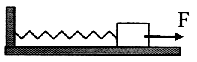
\includegraphics[width = 0.4 \textwidth]{ForceSpring.png}
\end{center}
\begin{ans}
$x = \frac{2F}{4\pi^2 \nu^2 m} = 25,3$ см, $x = v\sqrt{\frac{m}{k}}=15,9$ мм
\end{ans}
\end{ex}